\chapter{Sociophysics: Game Theory on networks}

\resp{Lorenzo Vigorelli}
 


\section{Ultimatum game}
The Ultimatum Game illustrates \cite{sinatra2009ultimatum} how fairness and the rejection of unfair offers can spread in a population, and it is often linked to the emergence of cooperation.  
It is a two-player game: the \emph{proposer} decides how to split a fixed reward $p$, while the \emph{responder} accepts if $p \geq q$ (strategy) or rejects otherwise. If accepted, the division is implemented, if rejected, both players receive zero payoff.  
The static (Nash) solution predicts that the proposer offers the minimum amount and the responder still accepts.  

\noindent On a network, each node represents a player who interacts with its neighbors, playing both roles. Three types of strategies are considered:  
\begin{itemize}
    \item \textbf{Fair}: $q = p$ (the player demands exactly what it offers);  
    \item \textbf{Pragmatic}: $q = 1-p$ (the player ensures the same payoff regardless of the role);  
    \item \textbf{Random}: $(p,q)$ chosen at random.  
\end{itemize}  

\noindent After each round, payoffs are compared and strategies evolve according to one of two rules:  
\begin{itemize}
    \item \textbf{Natural selection:} player $i$ compares its payoff $\Pi_i$ 
    with that of a neighbor $j$ and adopts $(p_j,q_j)$ with probability
    \begin{equation}
      P_{ij} = \frac{\Pi_j - \Pi_i}{2 \max \{ k_i, k_j \}}, \quad \text{if } \Pi_j > \Pi_i.
    \end{equation}

    \item \textbf{Social penalty:} the player with the lowest payoff and all its neighbors 
    are replaced by new players with random strategies, while keeping the same network connections.  
\end{itemize}



\section{Simulations}
Each network has been tested with both update rules (natural selection, social
penalty) and different player types (A, B, C, mixed). Three network topologies
were considered: Erdős-Rényi (ER), Barabási-Albert (BA), and an empirical
network (Karate Club).  
The following figures highlight the main effects of network structure, player
type, and update rule. The remaining cases are reported in the appendix \ref{app:ultimatum}.

\begin{figure*}[h!]
    \centering
    \setlength{\tabcolsep}{2pt}
    \begin{minipage}[t]{0.48\textwidth}
        \centering
        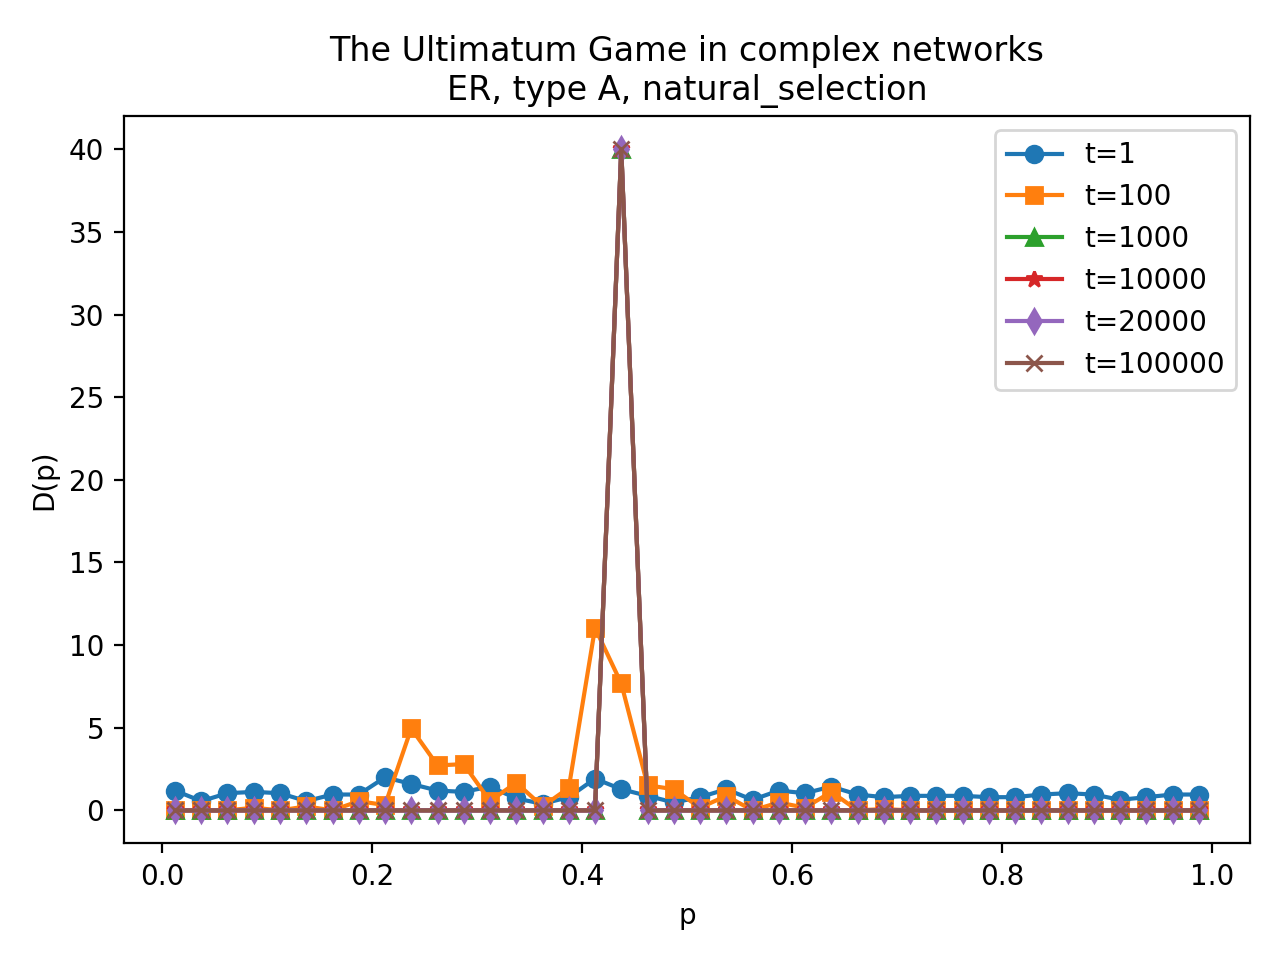
\includegraphics[width=\textwidth]{images/TASK1/Dp_ER_A_natural_selection.png}
        \subcaption{ER: $D(p)$ with central plateau}
        \label{fig:ER_Dp}
    \end{minipage}
    \hfill
    \begin{minipage}[t]{0.48\textwidth}
        \centering
        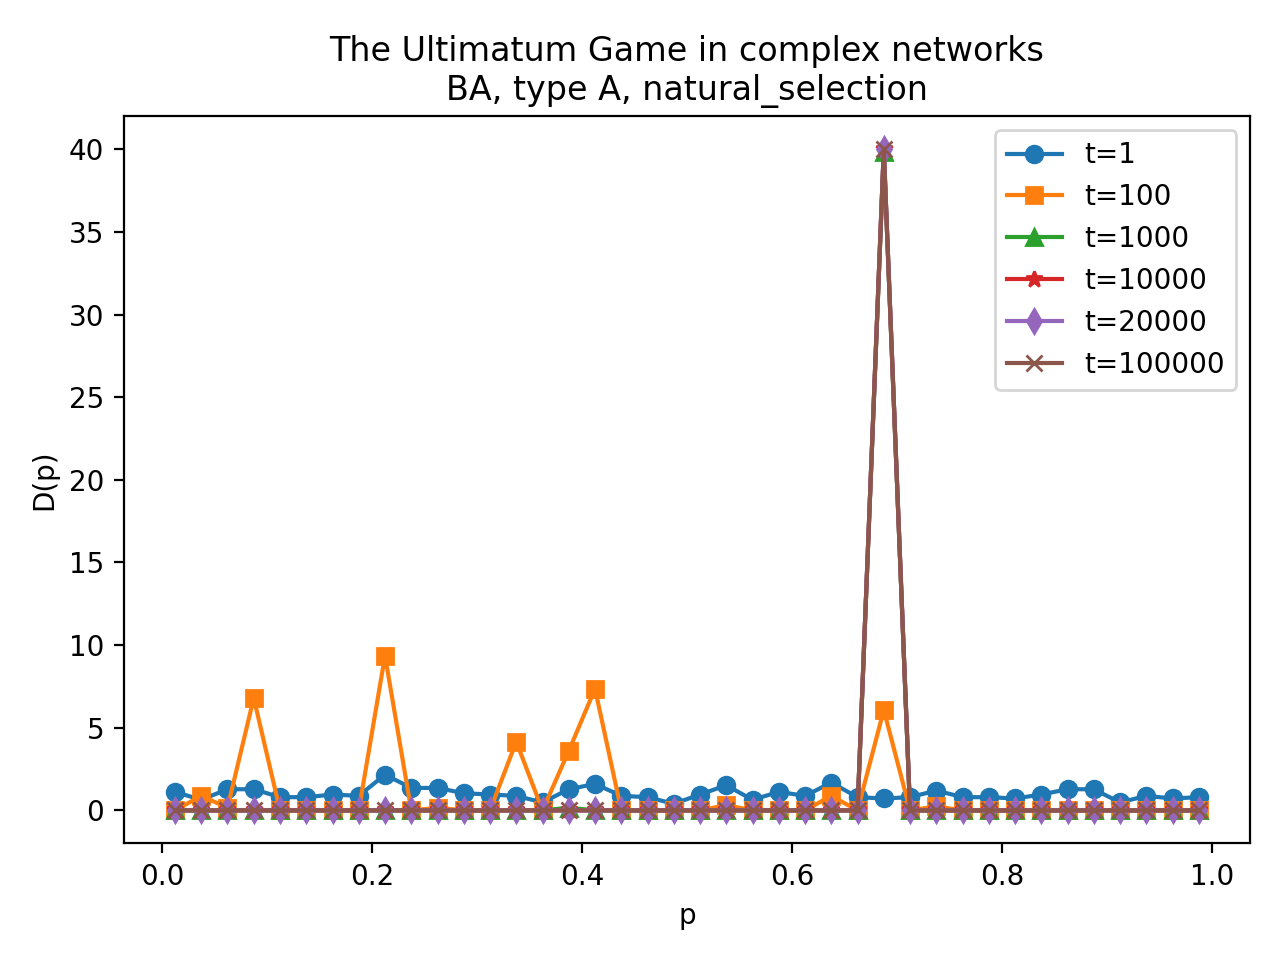
\includegraphics[width=\textwidth]{images/TASK1/Dp_BA_A_natural_selection.png}
        \subcaption{BA: $D(p)$ with shifted plateau (hubs)}
        \label{fig:BA_Dp}
    \end{minipage}
    \caption{Comparison of $D(p)$ in ER and BA networks under natural selection.}
    \label{fig:ER_BA_Dp}
\end{figure*}

\noindent\textbf{ER vs BA under natural selection.}  
Figure~\ref{fig:ER_BA_Dp} shows the contrast between homogeneous and scale-free
networks. In ER, strategies converge towards a stable plateau around
intermediate offers $p$, reflecting uniform connectivity.  
In BA, the presence of hubs shifts and distorts this plateau, producing sharper
peaks and greater heterogeneity. Overall, BA amplifies local instabilities,
while ER smooths strategies into collective equilibrium.

\begin{figure*}[h!]
    \centering
    \setlength{\tabcolsep}{2pt}
    \begin{minipage}[t]{0.48\textwidth}
        \centering
        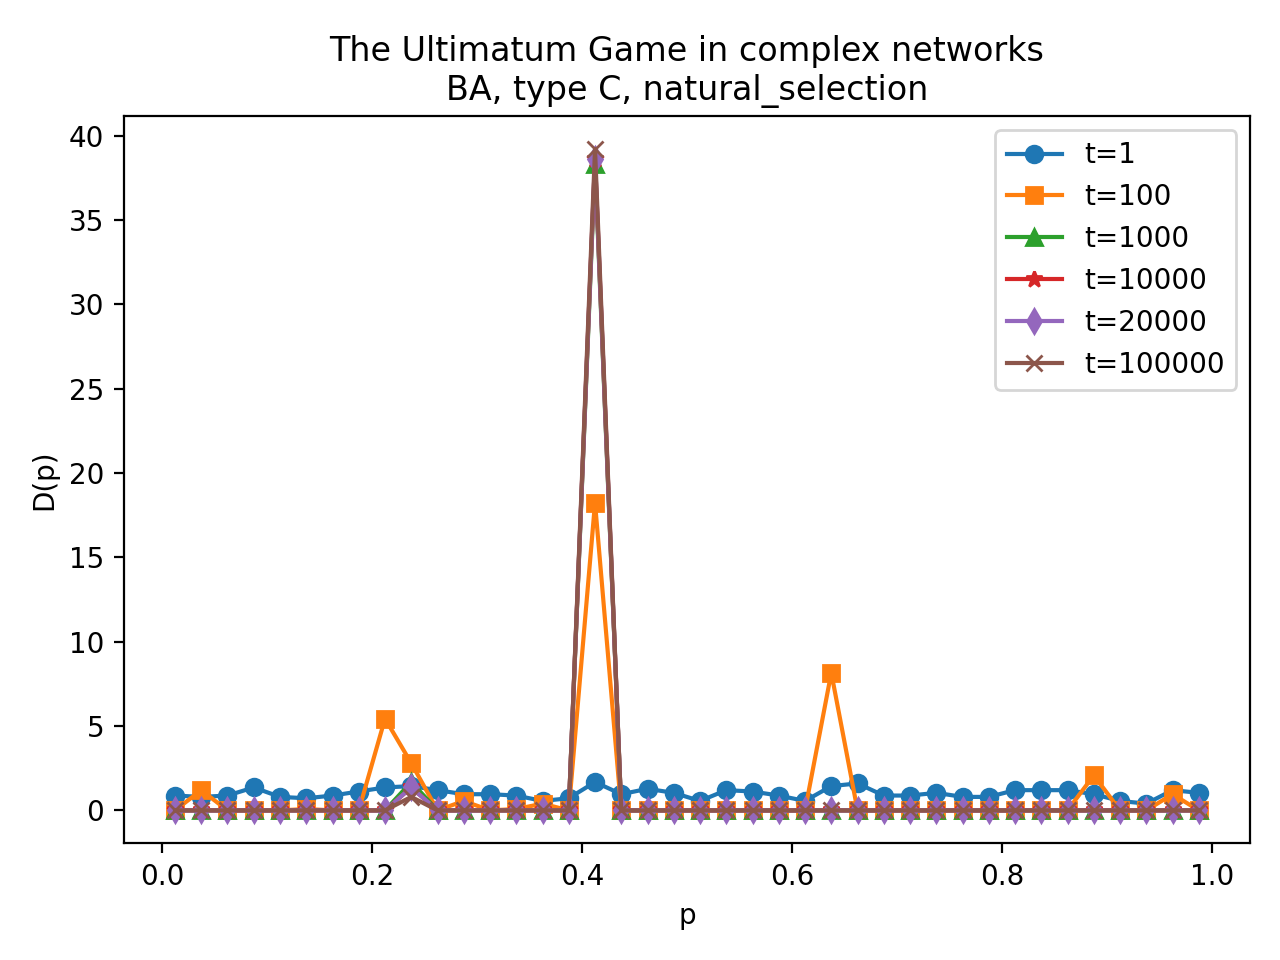
\includegraphics[width=\textwidth]{images/TASK1/Dp_BA_C_natural_selection.png}
        \subcaption{BA: $D(p)$.}
        \label{fig:BA_Dp_C}
    \end{minipage}
    \hfill
    \begin{minipage}[t]{0.48\textwidth}
        \centering
        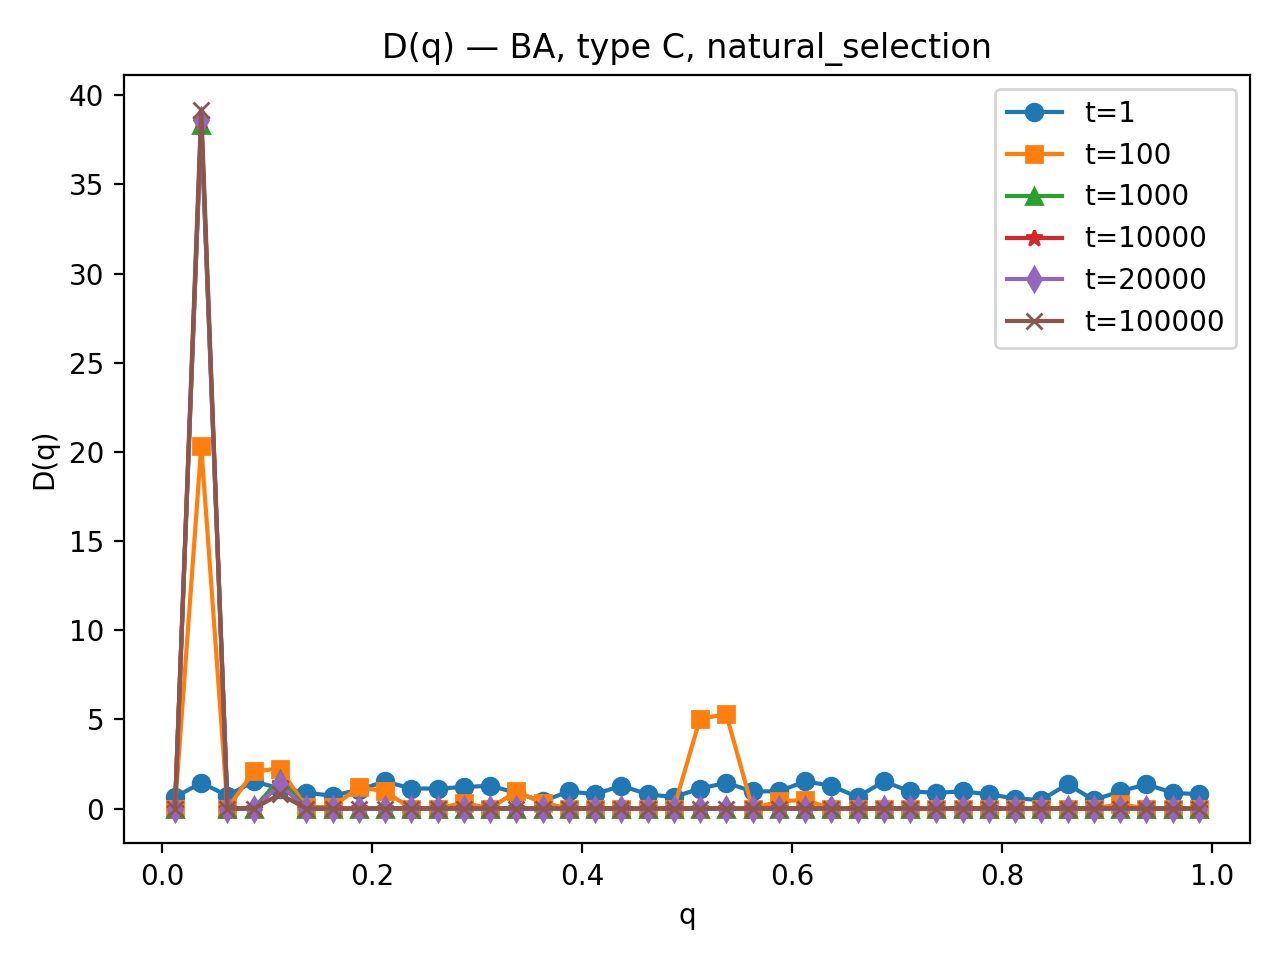
\includegraphics[width=\textwidth]{images/TASK1/Dq_BA_C_natural_selection.png}
        \subcaption{BA: $D(q)$.}
        \label{fig:BA_Dq_C}
    \end{minipage}
    \caption{Distributions of proposals ($p$) and acceptance thresholds ($q$) in BA network with random players under natural selection.}
    \label{fig:BA_pq_C}
\end{figure*}

\noindent\textbf{Asymmetry between proposals and acceptance (BA, C players).}  
Figure~\ref{fig:BA_pq_C} shows that proposals $p$ remain variable and
multimodal, stabilizing around several peaks (Fig.~\ref{fig:BA_Dp_C}), while
acceptance thresholds $q$ collapse to very low values
(Fig.~\ref{fig:BA_Dq_C}).  
This asymmetry reflects hub influence: they spread opportunistic acceptance
quickly, so even small offers are usually accepted, while offers themselves
retain heterogeneity.

\begin{figure*}[h!]
    \centering
    \setlength{\tabcolsep}{2pt}
    \begin{minipage}[t]{0.48\textwidth}
        \centering
        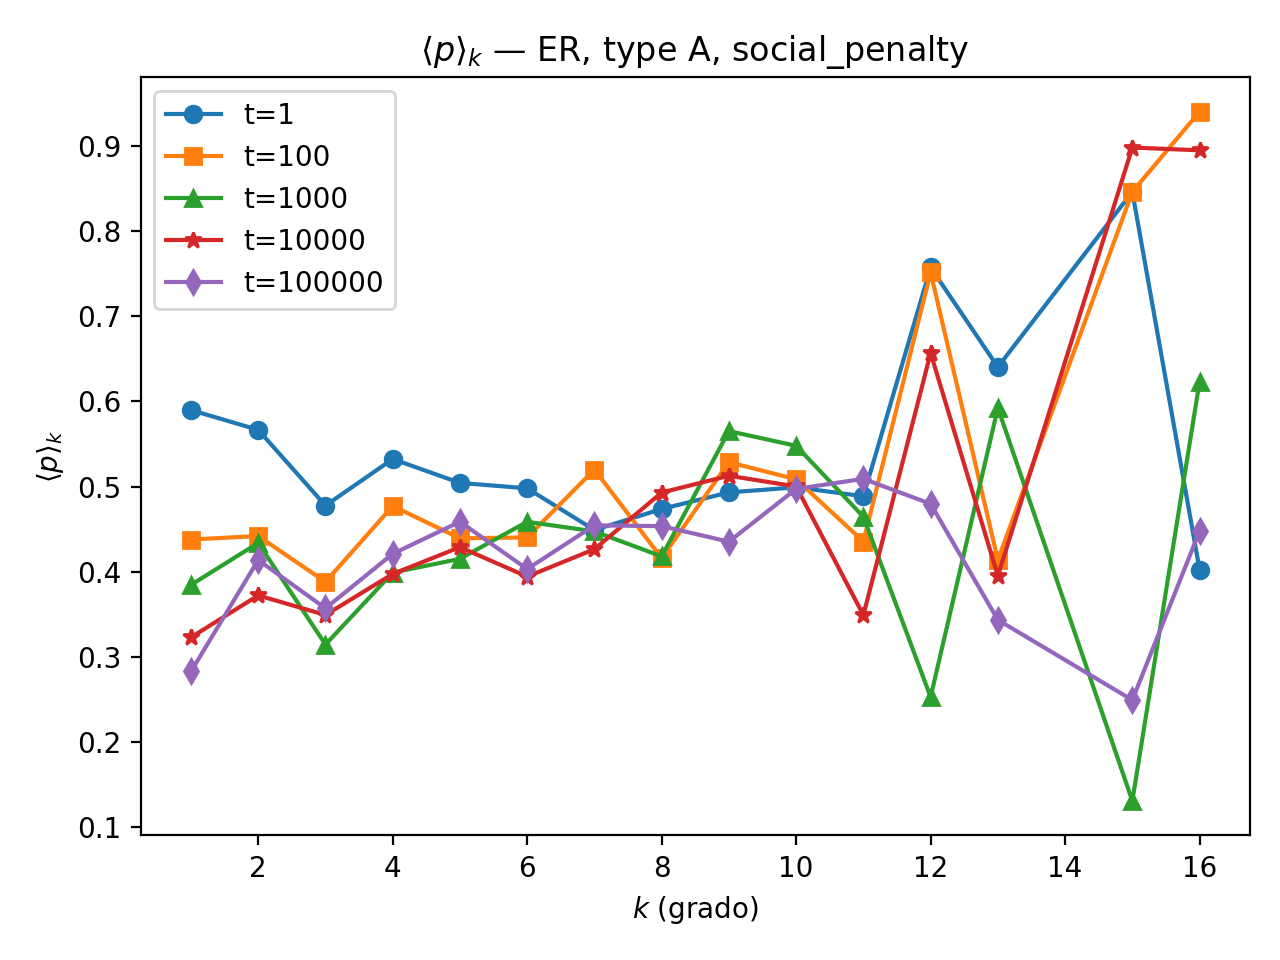
\includegraphics[width=\textwidth]{images/TASK1/p_by_degree_ER_A_social_penalty.png}
        \subcaption{Average proposal for A players}
        \label{fig:ER_lowdeg_p_SP}
    \end{minipage}
    \hfill
    \begin{minipage}[t]{0.48\textwidth}
        \centering
        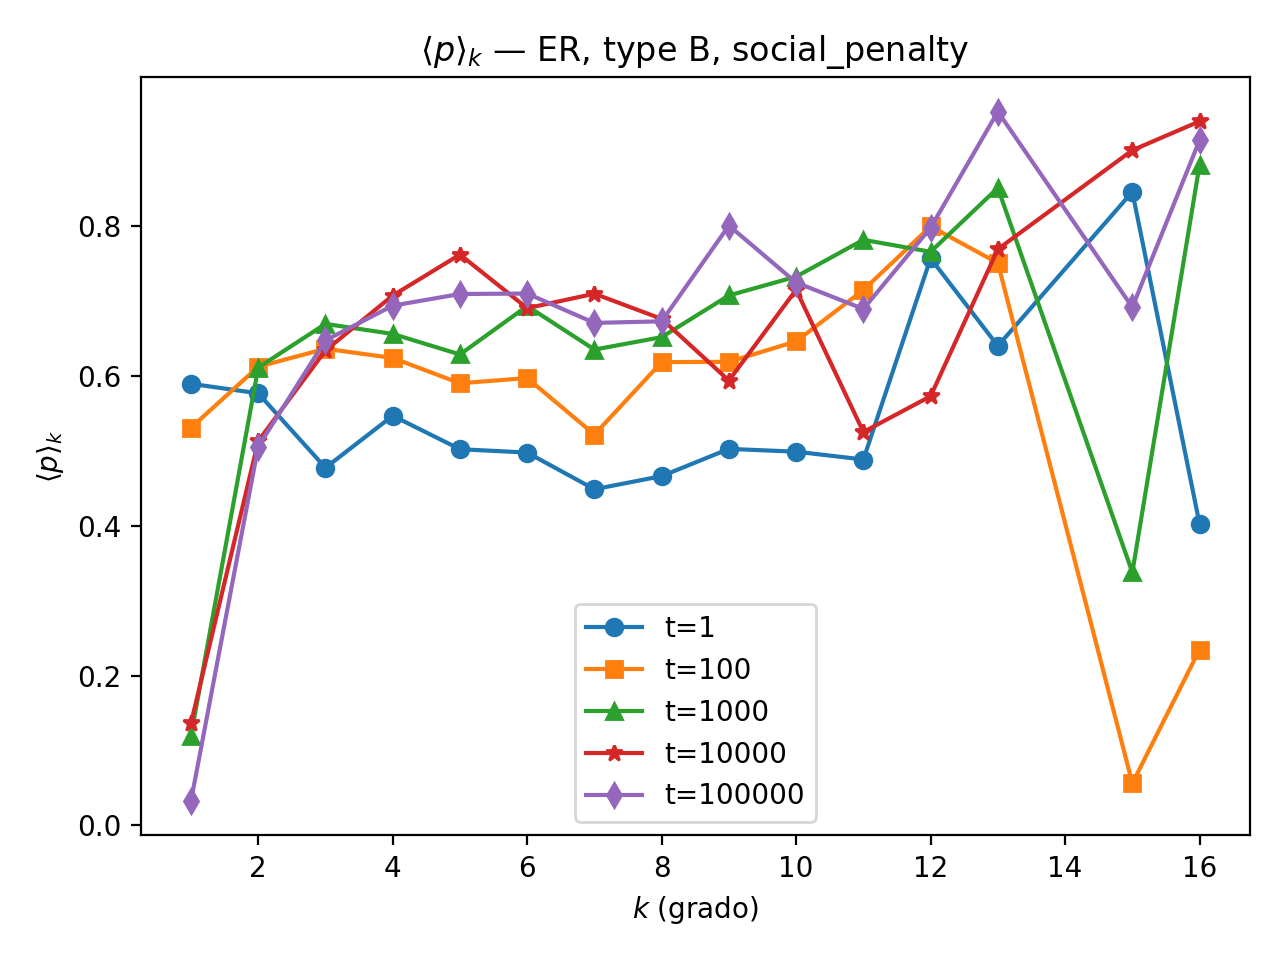
\includegraphics[width=\textwidth]{images/TASK1/p_by_degree_ER_B_social_penalty.png}
        \subcaption{Average proposal for B players}
        \label{fig:ER_highdeg_p_SP}
    \end{minipage}
    \caption{Average proposal $\langle p \rangle$ by node degree in ER network under social penalty.}
    \label{fig:ER_p_by_degree_SP}
\end{figure*}

\noindent\textbf{Social penalty and node degree.}  
Figure~\ref{fig:ER_p_by_degree_SP} illustrates the degree dependence under
social penalty. We show results by degree class because they highlight more
clearly the contrast between low- and high-connectivity players: global
distributions tend to hide these effects, while averages by degree reveal the
structural role of connectivity.  
For type A players (Fig.~\ref{fig:ER_lowdeg_p_SP}), low-degree nodes converge to
similar offers with only gradual adjustments.  
For type B players (Fig.~\ref{fig:ER_highdeg_p_SP}), convergence is slower and
more polarized: low-degree nodes end up offering very little, while high-degree
nodes move towards fairer offers.  
This strengthens heterogeneity and emphasizes that central nodes are pressured
into fairness, while peripheral ones remain selfish. Compared to natural
selection, convergence is slower and degree-based differences persist longer.



\section{Conclusions}

The simulations show that cooperation and fairness in the Ultimatum Game are
shaped by the interplay of network topology, player strategies, and update
rules.

\medskip
\noindent\textbf{Network topology.}  
ER networks smooth fluctuations and favor intermediate offers, while BA networks
amplify hub influence, producing heterogeneity and opportunistic acceptance.
Empirical networks display bimodal outcomes tied to community structure and
degree.

\medskip
\noindent\textbf{Player type.}  
Fair players (A) converge to intermediate offers in homogeneous settings but
become asymmetric in heterogeneous ones.  
Pragmatic players (B) show strong degree effects: low-degree nodes offer very
little, while hubs adopt fairer values.   Random players (C) generate multimodal proposals, with acceptance thresholds collapsing to low values.

\medskip
\noindent\textbf{Update rule.}  
Natural selection drives faster convergence and more uniform equilibria.  
Social penalty converges more slowly but enforces degree-based differentiation,
with high-degree nodes pressured into fairness and peripheral ones remaining
selfish.\\

\noindent\medskip
Fairness emerges not from strategies alone but from how they interact with network structure and update rules, with hubs acting as decisive drivers of global outcomes.

\newpage